\begin{appendix}
\chapter{Anhang}
\label{chap:anhang}

\section{Flächenflugzeug}
\label{sec:herleitung_geschw_bez}
Der in Gleichung \ref{eq:geschw_flaechenflugzeug} aufgeführte Zusammenhang entsteht aus dem Verhältnis der Fluggeschwindigkeiten bei konstanten Auftriebsbeiwert. Aus der Definition des Auftriebsbeiwertes
\begin{equation}
	c_{A} = \frac{A}{\rho/2\cdot V^2\cdot S}
\end{equation}
entsteht durch Umformen die Beziehung für die Geschwindigkeit
\begin{equation}
	V = \sqrt{\frac{2\cdot A}{\rho\cdot S \cdot c_{A}}} \eqend{.}
\end{equation}
Im Horizontalflug (\ensuremath{\gamma = 0}) kompensiert der Auftrieb lediglich die Gewichtskraft (Vgl. Gleichung \ref{eq:auftriebsgleichung_vereinfacht})
\begin{equation}
	A = G \eqend{.}
\end{equation}
Für jegliche Art von Steigflug (\ensuremath{\gamma \neq 0}) ist dies nicht mehr der Fall. Unter der Voraussetzung einer gleichen Gewichtskraft \ensuremath{m\cdot g}, gleicher Flügelfläche \ensuremath{S} und einem konstanten Auftriebsbeiwert \ensuremath{c_{A}} ergibt sich für das Verhältnis der Geschwindigkeiten \ensuremath{V/V^\star}
\begin{equation}
	\frac{V}{V^\star} = \frac{\sqrt{\frac{2\cdot m \cdot g\cdot \cos\gamma}{\rho\cdot S \cdot c_{A}}}}{\sqrt{\frac{2\cdot m\cdot g}{\rho^\star \cdot S \cdot c_{A}}}} = \sqrt{\cos\gamma\cdot\frac{\rho^\star}{\rho}} \eqend{.}
\end{equation}\\

\section{Propeller}
\label{sec:propellerkennfeld}
In Abb. \ref{abb:propellerkennfeld} ist beispielhaft das Kennfeld von einem APC 10x3 Propeller dargestellt. 
\begin{figure}[H]
\centering
	\includegraphics[scale=0.7]{Diagramme/Propellerkennfeld.pdf}
	\caption{beispielhaftes Propellerkennfeld für einen APC 10x3 Propeller}
	\label{abb:propellerkennfeld}
\end{figure}

\section{Motor}
\label{sec:motormodell}
Das Motormodell weist eine über das ganze Spektrum der möglichen Betriebspunkte konsistente Verteilung des Motorwirkungsgrades auf (Vgl. Abb. \ref{abb:motormodell}). Der maximale Motorwirkungsgrad wird bei maximaler Spannung und bei maximalen Strom erreicht. Der errechnete Wert stimmt mit einer Genauigkeit von \ensuremath{\pm \SI{2}{\%}} mit den Angaben vom Hersteller überein \cite{axi}.
\begin{figure}[H]
\centering
	\includegraphics[scale=0.7]{Diagramme/Motormodell.pdf}
	\caption{Wirkungsgrad aufgetragen über verschiedenen Betriebspunkten des Motors}
	\label{abb:motormodell}
\end{figure}

\section{Motorregler}
\label{sec:motorreglermodell}
Das Modell des Motorreglerwirkungsgrades ist in Abb. \ref{abb:motorreglermodell} dargestellt. Es zeigt den Wirkungsgrad des Motorreglers in Abhängigkeit der PWM. An dieser Stelle ist die ausschließliche Abhängigkeit des Modells von der PWM ersichtlich.
 
\begin{figure}[H]
\centering
	\includegraphics[scale=0.7]{Diagramme/Motorreglermodell.pdf}
	\caption{Wirkungsgrad des Motorreglers aufgetragen über der PWM}
	\label{abb:motorreglermodell}
\end{figure}


\section{Batteriekapazität}
Für die Untersuchungen ist eine Berechnung der Batteriekapazität unabhängig von der Art der Zelle, aber abhängig von der Batteriemasse von Interesse.
Aus diesem Grund bietet sich die Energiedichte an. 
Mit dieser berechnet sich die Kapazität wie folgt:
\begin{equation}
	C_{Bat}	= \omega\cdot\frac{m_{Bat}}{U_{Bat,nom}} \eqend{.}
	\label{eq:batteriekapazitaet}
\end{equation}


\section{Vergleich von normierter zur originalen Batteriezelle}
\label{sec:norm_vs_orig}
Für den Vergleich der Norm- mit der Originalzelle wird das Integral unterhalb der beiden Entladekurven für eine bestimmte Entladerate gebildet. Anschließend werden beide Flächen zueinander in Beziehung gesetzt 
\begin{equation}
	\text{Toleranz} = \frac{\text{F}_{Orig.}-\text{F}_{Norm}}{\text{F}_{Norm}} \eqend{.}
\end{equation} 
Im Sinne einer Genauigkeitssteigerung werden alle die Batterien in der Normzellenberechnung nicht berücksichtigt, deren individuelle Abweichung eine große Diskrepanz zur Standardabweichung aufweist. Der Vergleich zeigt, dass es starke Abweichungen bei den Batterien gibt. Die durchschnittliche Abweichung liegt für Entladeraten bis \SI{45}{1/h} deutlich über Null und steigt mit der Entladerate von \SI{8}{\%} auf \SI{17}{\%} bei \SI{45}{1/h}. Die Spannung der Normzelle ist somit im Durchschnitt kleiner als die der originalen Batteriezelle (Vgl. Abb. \ref{abb:batterie_abweichungen}). Ab der Entladerate von \SI{50}{1/h} fällt die Abweichung drastisch auf \SI{-18}{\%} ab. 
\begin{figure}[H]
\centering
	\includegraphics[scale=0.7]{Diagramme/Abweichungen.pdf}
	\caption{links: Durchschnittliche Spannungsabweichungen der Normzelle von den Zellen aus der Batteriedatenbank in Abhängigkeit von der C-Rate,\\ rechts: Beispiel für die Spannungsabweichungen jeder Normzelle im Vergleich zur Originalzelle für eine Entladerate von \SI{20}{1/h}
	 }
	\label{abb:batterie_abweichungen}
\end{figure}


\section{Steiggeschwindigkeit}
\label{sec:vvar_vorgehen}

\begin{center}
\begin{figure}[H]
\begin{struktogramm}(163,160)
\while[5]{Für alle Bahngeschwindigkeiten}
	\assign[2]{Berechne Gesamtmasse}
	\assign[2]{Flugzeit für Höhenschritt berechnen}			
	\while[5]{Solange Abbruchkriterium nicht erreicht}
		\assign{Aerodynamik berechnen}
	\whileend
	\assign[2]{Schub berechnen}
	\assign[2]{Schub auf Propeller verteilen}
	\ifthenelse[10]{1}{4}{Schub zu gro\ss{}?}{ja}{nein}
		\assign[2]{Ergebnis verwerfen (NaN)}
		\change
		\assign[2]{Drehzahl und Drehmoment aus Propellerkennfeld interpolieren}
		\assign[2]{Motorzustand berechnen}
		\assign[2]{Zustand der Motorregler berechnen}
		\assign[2]{Zustand der Batterie neu berechnen}
		\assign[2]{Gesamtwirkungsgrad berechnen}
	\ifend
	\ifthenelse[10]{1}{1}{Werden Grenzen überschritten?}{ja}{nein}
		\assign[2]{Ergebnis verwerfen (NaN)}
		\change
		\assign[2]{Ergebnis beibehalten}
	\ifend
	\assign[2]{Speichern der aufgebrachten Energiemenge}
\whileend
\ifthenelse[10]{5}{1}{Sind die Werte NaN?}{nein}{ja}
	\while[5]{Solange Abbruchkriterium nicht erreicht}		
		\assign[2]{Finde den Index mit der geringsten verbrauchten Energiemenge}
		\ifthenelse[10]{1}{3}{Werte innerhalb Leistungsgrenzen?}{ja}{nein}
			\assign[2]{Verlasse Schleife}
			\change
			\assign[2]{Suche nächst kleinere Energiemenge}
		\ifend
	\whileend
	\assign[2]{Übergabe aller Leistungsparameter mit diesem Index}
		\change
	\assign[2]{Verwerfe alle Ergebnisse}
\ifend
\end{struktogramm}
\caption{Programmstruktur zur Ermittlung der optimalen Steiggeschwindigkeit}
\label{abb:steiggeschw}
\end{figure}
\end{center}

\section{Motorreglerwirkungsgrad}
\label{sec:motorreglerwirkungsgrad}

Im Folgenden ist der Einfluss des ESC-Wirkungsgrades auf den TOC veranschaulicht. Dafür werden zwei Batteriegrößen untersucht, eine mit sechs Zellen und einmal mit acht Zellen. Die Masse und Kapazität bleiben jeweils gleich. 

\begin{figure}[H]
\centering
	\includegraphics[scale=0.7]{Diagramme/Untersuchung_eta_pwm_normal_6.pdf}
	\caption{Leistungsparameter der Multicopter-Referenzkonfiguration (vgl. Tab. \ref{tab:referenzkonfiguration_mulitcopter}) für den Motorreglerwirkungsgrades für eine Batterie mit sechs Zellen}
	\label{abb:eta_pwm_6_normal}
\end{figure}

\begin{figure}[H]
\centering
	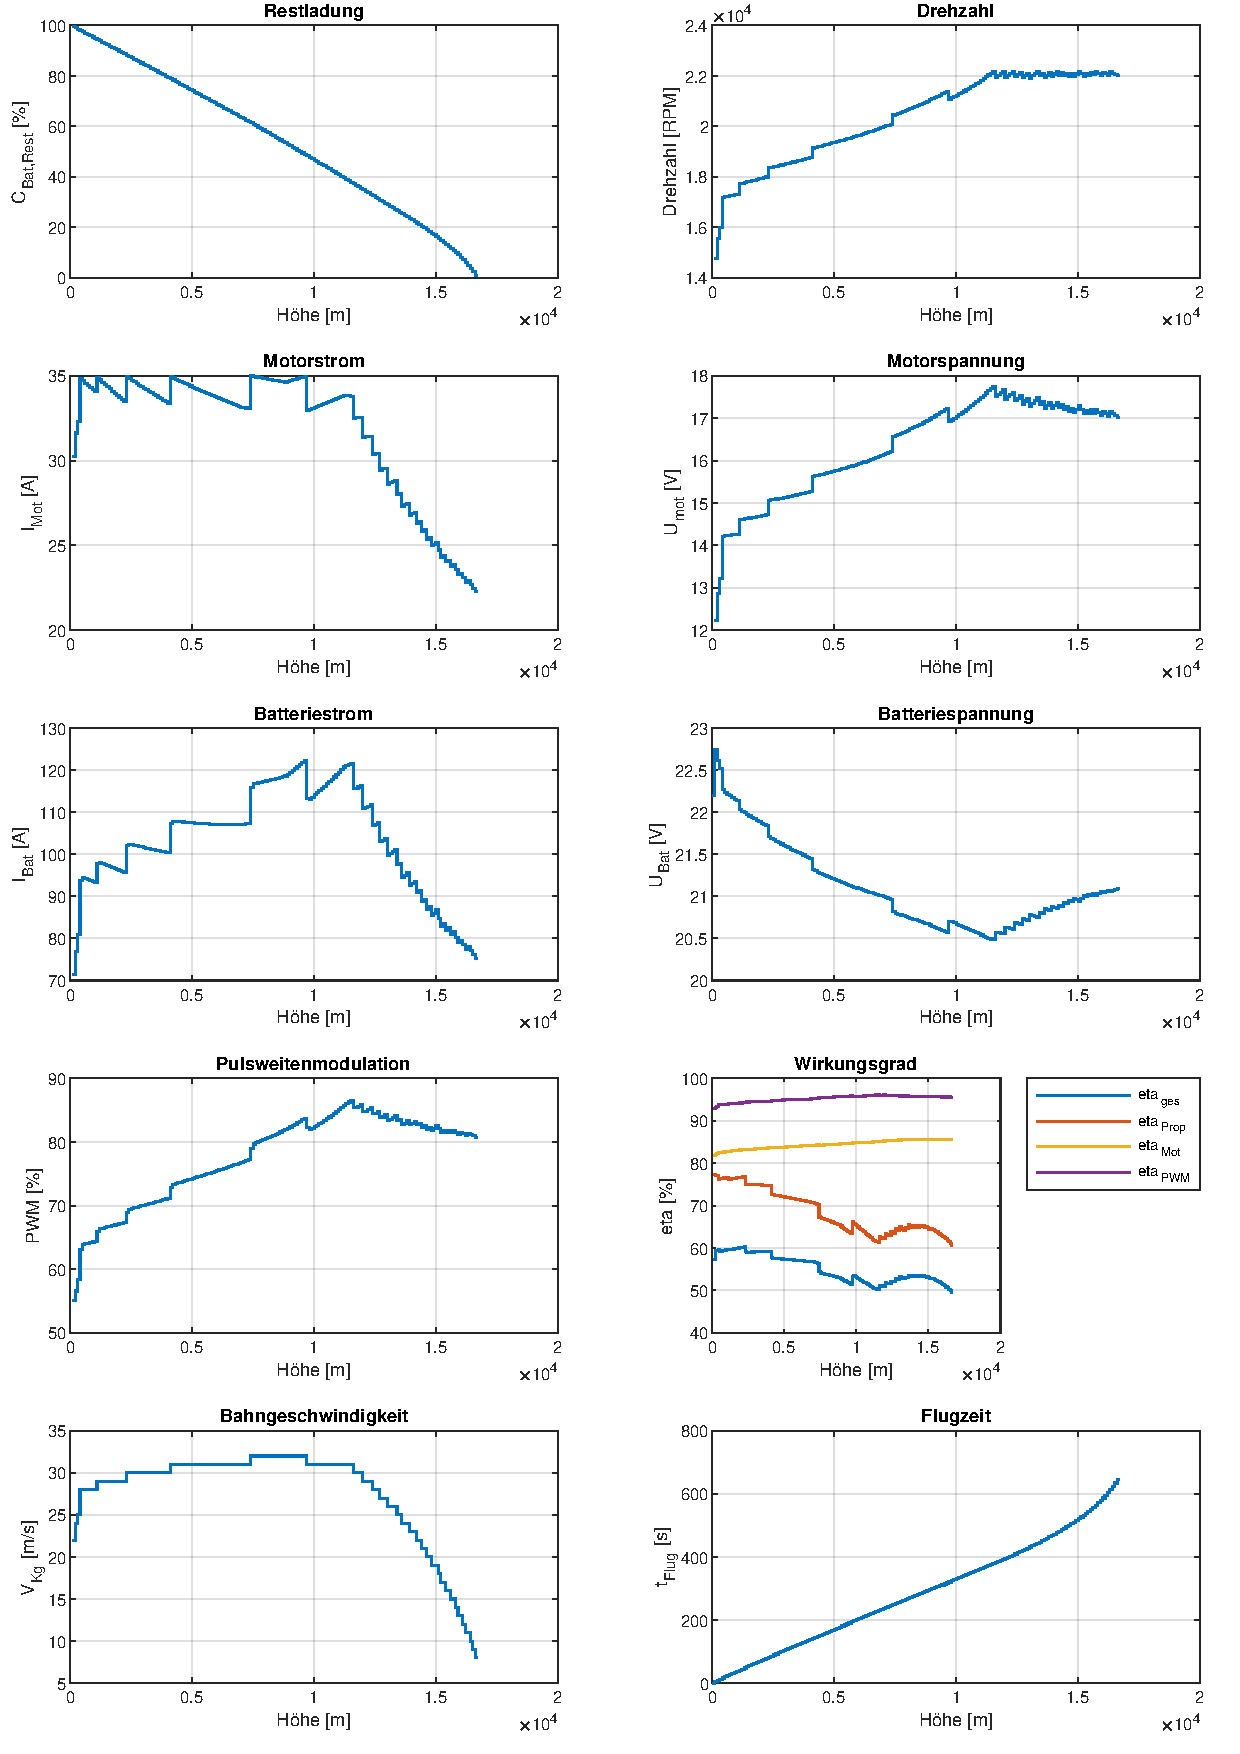
\includegraphics[scale=0.7]{Diagramme/Untersuchung_eta_pwm_halbierung_6.pdf}
	\caption{Leistungsparameter der Multicopter-Referenzkonfiguration (vgl. Tab. \ref{tab:referenzkonfiguration_mulitcopter}) für eine Verbesserung des Motorreglerwirkungsgrades (Halbierung der Verluste) für eine Batterie mit sechs Zellen}
	\label{abb:eta_pwm_6_halb}
\end{figure}

\begin{figure}[H]
\centering
	\includegraphics[scale=0.7]{Diagramme/Untersuchung_eta_pwm_1_6.pdf}
	\caption{Leistungsparameter der Multicopter-Referenzkonfiguration (vgl. Tab. \ref{tab:referenzkonfiguration_mulitcopter}) für eine Verbesserung des Motorreglerwirkungsgrades (keine Verluste) für eine Batterie mit sechs Zellen}
	\label{abb:eta_pwm_6_1}
\end{figure}


\section{Batteriemasse}
\label{sec:batteriemasse}
Es zeigt sich, dass das Optimum des Batteriemassenanteils bei \SI{66.66}{\%} oder leicht darunter liegt. Eine Erhöhung führt zu schlechteren Flugleistungen und einem schnelleren Absinken der Restkapazität gegen Null (vgl. Abb. \ref{abb:batteriemasse_genauer}). Deutlich ist zudem der Einfluss der Batteriemasse auf die Bahngeschwindigkeit gegeben. Mit der Masse sinkt die optimale Bahngeschwindigkeit. 
\begin{figure}[H]
\centering
	\includegraphics[scale=0.7]{Diagramme/Batteriemasse_genauer.pdf}
	\caption{genauere Untersuchung der Batteriemassenabhängigkeit (\ensuremath{m_{Mot}=\SI{106}{g}}, \ensuremath{K_V=\SI{1390}{RPM/V}}, \ensuremath{n_{Prop}=4}, \ensuremath{Propeller=\SI{10x3}{}}, \ensuremath{n_{Bat,cell}=4}, \ensuremath{u_{Wg}=\SI{10}{m/s}})}
	\label{abb:batteriemasse_genauer}
\end{figure}

\section{Verstellpropeller}
\label{sec:vprop_vorgehen}
In Abb. \ref{abb:vpp_vorberechnung} ist die Entnahme aller Kennfelder mit dem vorgegeben Durchmesser dargelegt. Im Anschluss folgt die Flugleistungsberechnung für einen Multicopter mit Verstellpropeller in Abb. \ref{abb:vpp_flugleistungsberechnung}.
\begin{center}
\begin{figure}[H]
\begin{struktogramm}(163,70)
\assign[1]{Multicopter- und Umgebungsparameter festlegen (im Startskript)}
\assign[1]{Diskretisierungen (Geschwindigkeit, Höhe) festlegen}
\assign[1]{Aufruf des Hauptskripts: Leistungsberechnung starten}
\while[5]{Für alle Zeilen der APC-Datenbank}
	\ifthenelse[10]{1}{1}{Stimmt Durchmesser mit dem gesuchten überein?}{ja}{nein}
		\assign[2]{Gehe zur nächsten Zeile}
		\change
		\assign[2]{Lösche Zeile}
	\ifend
\whileend
\while[5]{Für alle Propeller}
	\assign[2]{Extrahiere Propellerkennfeld}
	\assign[2]{Speicher das Ergebnis unter fortlaufenden Nummern}
	\assign[2]{Erhöhe Propellerzähler}
\whileend
\end{struktogramm}
\caption{Programmstruktur für die Entnahme aller Propellerkennfelder mit dem zu untersuchenden Durchmesser}
\label{abb:vpp_vorberechnung}
\end{figure}
\end{center}

\begin{center}
\begin{figure}[H]
\begin{struktogramm}(163,210)
\assign[1]{Initialisierung der Parameterberechnung}
\while[5]{F\"ur alle Höhenabschnitte}
	\assign[1]{H\"ohe, Dichte, Luftdruck Temperatur berechnen}
	\assign[1]{Berechnung des arithmetischen Mittelwertes}
	\assign[1]{Schub- und Leistungskennfeld anpassen}
	\assign[2]{Initialisierung der Leistungsberechnung}
	\while[5]{Für alle Bahngeschwindigkeiten}
		\assign[2]{Initialisierungen}
		\while[5]{Für alle Propeller}
			\assign[2]{\texttt{\textbf{Leistungsberechnung}}}
			\assign[2]{Berechnung benötigter Energiemenge bei dieser Bahngeschwindigkeit mit diesem Propeller}
		\whileend
		\ifthenelse[10]{4}{1}{Sind die Werte NaN?}{nein}{ja}
			\while[5]{Solange Abbruchkriterium nicht erreicht}		
				\assign[2]{Finde den Index mit der geringsten verbrauchten Energiemenge}
				\ifthenelse[10]{1}{1}{Werte innerhalb Leistungsgrenzen?}{ja}{nein}
				\assign[2]{Verlasse Schleife}
				\change
				\assign[2]{Suche nächst kleinere Energiemenge}
				\ifend
			\whileend
			\assign[2]{Übergabe aller Leistungsparameter mit diesem Index}
			\change
			\assign[2]{Verwerfe alle Ergebnisse}
		\ifend
		\assign[2]{Berechne benötigte Energie für Steiggeschwindigkeit}
	\whileend
	\ifthenelse[10]{4}{1}{Sind die Werte NaN?}{nein}{ja}
		\while[5]{Solange Abbruchkriterium nicht erreicht}		
			\assign[2]{Finde den Index mit der geringsten verbrauchten Energiemenge}
			\ifthenelse[10]{1}{1}{Werte innerhalb Leistungsgrenzen?}{ja}{nein}
			\assign[2]{Verlasse Schleife}
			\change
			\assign[2]{Suche nächst kleinere Energiemenge}
			\ifend
		\whileend
		\assign[2]{Übergabe aller Leistungsparameter mit diesem Index}
		\change
		\assign[2]{Verwerfe alle Ergebnisse}
	\ifend
	\assign[2]{Erhöhe Zählervariable}
\whileend
\assign[2]{Ergebnisse der Leistungsparameter in Diagrammen speichern}
\assign[2]{Speichern der Diagramme in .pdf-Datei}
\end{struktogramm}
\caption{Programmstruktur für die Untersuchung des Nutzens eines Verstellpropellers}
\label{abb:vpp_flugleistungsberechnung}
\end{figure}
\end{center}

Der Verlauf des Gesamtwirkungsgrades folgt eindeutig dem Verlauf des Propellerwirkungsgrades. Dieser ist die Ursache für den höheren Gesamtwirkungsgrad des Verstellpropellers (Vgl. Abb. \ref{abb:verstellprop_eta}).

\begin{figure}[H]
\centering
	\includegraphics[scale=0.7]{Diagramme/Verstellprop_eta.pdf}
	\caption{Einfluss des Verstellpropellers auf die maximal erreichbare Höhe mit besonderem Hinblick auf die Einzelwirkungsgrade}
	\label{abb:verstellprop_eta}
\end{figure}

In Abb. \ref{abb:verstellprop_real} ist der Gewichtseinfluss auf die Flugleistungen eines Multicopters mit Verstellpropeller dargestellt. Das Gewicht verringert die Flugleistungen deutlich. Außerdem kann für die Referenzkonfiguration festgehalten werden, dass der Vorteil des Verstellpropellers bei einem Gewicht des Verstellmechanismus von \SI{85}{g} pro Propeller kompensiert wird. Insgesamt ergibt dies einen Anteil von ca. \SI{10}{\%} am Gesamtgewicht. Wird dieser Anteil überschritten, ist der Nutzen des Verstellpropeller nichtig. Alle Gewichtsanteile darunter ergeben einen Nutzen. 
\begin{figure}[H]
\centering
	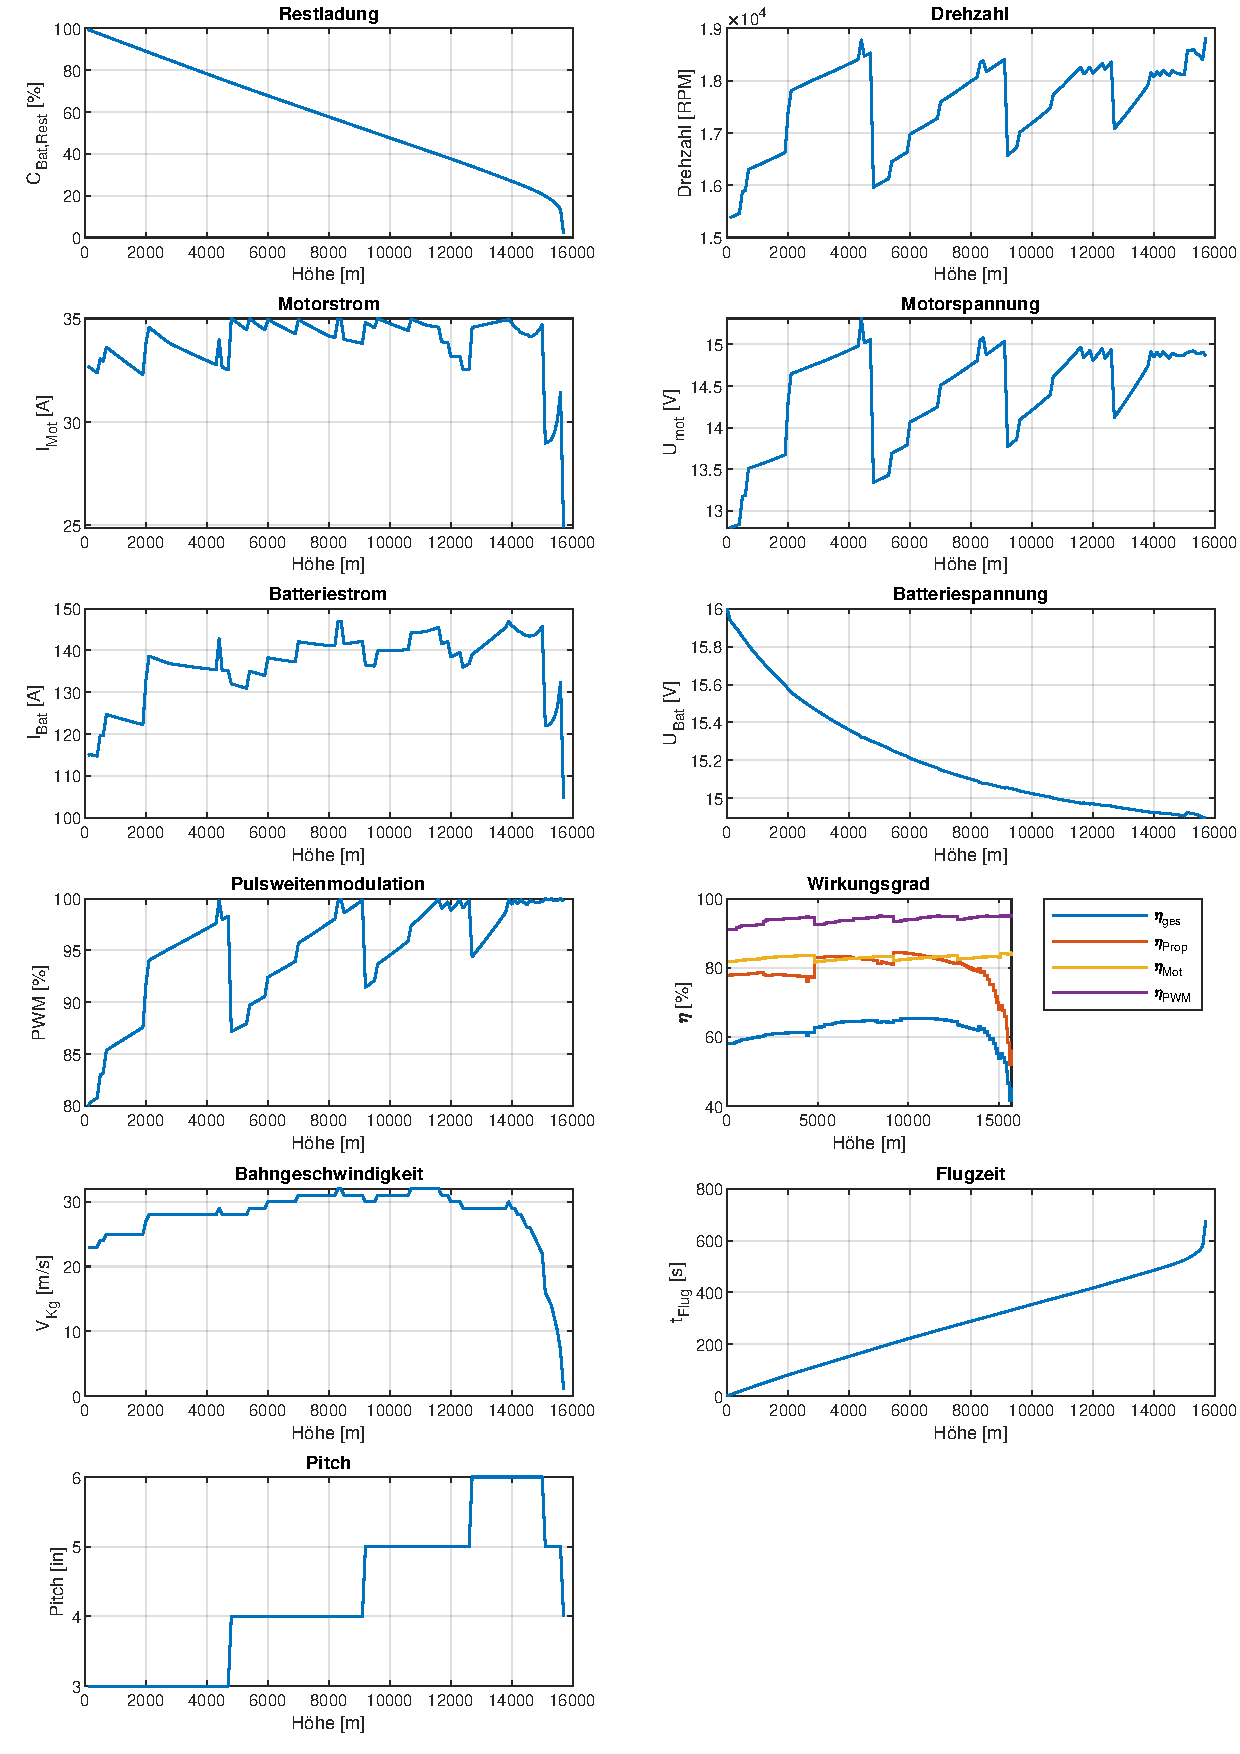
\includegraphics[scale=0.7]{Diagramme/Verstellprop_real.pdf}
	\caption{Einfluss des Verstellpropellers auf die Flugleistungen der Referenzkonfiguration des Multicopters mit einem Gewicht von \SI{85}{g} pro Verstelleinrichtung}
	\label{abb:verstellprop_real}
\end{figure}


\section{Getriebe}
\label{sec:getriebe_vorgehen}
\begin{center}
\begin{figure}[H]
\begin{struktogramm}(163,210)
\assign[1]{Multicopter- und Umgebungsparameter festlegen (im Startskript)}
\assign[1]{Diskretisierungen (Getriebe, Geschwindigkeit, Höhe) festlegen}
\assign[1]{Aufruf des Hauptskripts: Leistungsberechnung starten}
\assign[1]{Initialisierung der Parameterberechnung}
\while[5]{F\"ur alle Höhenabschnitte}
	\assign[1]{H\"ohe, Dichte, Luftdruck Temperatur berechnen}
	\assign[1]{Berechnung des arithmetischen Mittelwertes}
	\assign[1]{Schub- und Leistungskennfeld anpassen}
	\assign[2]{Initialisierung der Leistungsberechnung}
	\while[5]{Für alle Bahngeschwindigkeiten}
		\assign[2]{Initialisierungen}
		\while[5]{Für alle Übersetzungen}
			\assign[2]{\textbf{Leistungsberechnung}}
		\whileend
		\ifthenelse[10]{4}{1}{Sind die Werte NaN?}{nein}{ja}
			\while[5]{Solange Abbruchkriterium nicht erreicht}		
				\assign[2]{Finde den Index mit der geringsten verbrauchten Energiemenge}
				\ifthenelse[10]{1}{1}{Grenzen überschritten?}{nein}{ja}
				\assign[2]{Verlasse Schleife}
				\change
				\assign[2]{Suche nächst kleineren Energiemenge}
				\ifend
			\whileend
			\assign[2]{Übergabe aller Leistungsparameter mit diesem Index}
			\change
			\assign[2]{Verwerfe alle Ergebnisse}
		\ifend
		\assign[2]{Berechne benötigte Energie für Steiggeschwindigkeit}
	\whileend
	\ifthenelse[10]{4}{1}{Sind die Werte NaN?}{nein}{ja}
		\while[5]{Solange Abbruchkriterium nicht erreicht}		
			\assign[2]{Finde den Index mit der geringsten verbrauchten Energiemenge}
			\ifthenelse[10]{1}{1}{Grenzen überschritten?}{nein}{ja}
			\assign[2]{Verlasse Schleife}
			\change
			\assign[2]{Suche nächst kleinere Energiemenge}
			\ifend
		\whileend
		\assign[2]{Übergabe aller Leistungsparameter mit diesem Index}
		\change
		\assign[2]{Verwerfe alle Ergebnisse}
	\ifend
	\assign[2]{Erhöhe Zählervariable}
\whileend
\assign[2]{Ergebnisse der Leistungsparameter in Diagrammen speichern}
\assign[2]{Speichern der Diagramme in .pdf-Datei}
\end{struktogramm}
\caption{Programmstruktur die Untersuchung des Nutzens eines Getriebes}
\label{abb:getriebe_struktogramm}
\end{figure}
\end{center}

\section{Einfluss der Nutzlast}
\label{sec:einfluss_nutzlast}
Auf eine Reduzierung der Batteriemasse durch die zusätzliche Nutzlast wird in Kap. \ref{subsec:aeromet_rb} bewusst verzichtet. Der Vergleich von Abb. \ref{abb:aeromet_rb} mit Abb. \ref{abb:aeromet_rb_batterie_redu} zeigt auf, dass eine Reduzierung der Gesamtmasse im Sinne einer Schubsenkung wenig Einfluss auf die Flugleistungen hat. Dies bestätigt die Aussage aus Abschn. \ref{subsec:groesse}. Der Einfluss der Nutzlast mit konstanten \SI{250}{g} nimmt ab, je kleiner deren Anteil an der Gesamtmasse ist.  

\begin{figure}[H]
\centering
	\includegraphics[scale=0.7]{Diagramme/aeromet_nutzlast_redu.pdf}
	\caption{Einfluss der Batteriemassenreduzierung durch die Nutzlast auf die Flugleistungen der optimalen Lösung (vgl. Tab. \ref{tab:optimale_konfiguration})}
	\label{abb:aeromet_rb_batterie_redu}
\end{figure}



\end{appendix}
